\chapter{The CLAS12 Drift Chamber}

\section{Overview}

The CLAS12 Drift Chamber (DC) is a subsystem of the CLAS12 particle
detector, located inside one of the halls of the Thomas
Jefferson National Facility, Newport News Virginia, U.S.A. The
detector is used at the core of many experiments, designed to gather
information on particle interactions, mostly originating from an
electron beam hitting a target inside of its center.

After interacting with the target, the resulting particles pass
through the drift chamber subsystem that is designed to measure their
momentum, which is done to aquire further insights into the underlying
physical processes. This core responsibility of the drift chamber to
register the results of particle interaction is the reason why it is
deemed to be the most crucial component of the CLAS12 particle
detector.

\section{Layout}

The drift chamber itself is composed of a hierarchical arrangement of
single wires, where each wire is responsible for detecting the presence of
particles by emiting signals of activation. It consists of 18
individual wire chambers, each made up of two superlayers. A
superlayer is a collection of six simple layers, each consisting of
112 wires, which means that the whole system contains a total of
\(112 \cdot 6 \cdot 2 \cdot 18 = 24,192\) wires.
A visual representation of the hierarchical structure of a
single wire chamber can be found in Fig. \ref{fig:wire-chamber}.
\begin{figure}[h]
  \centering
  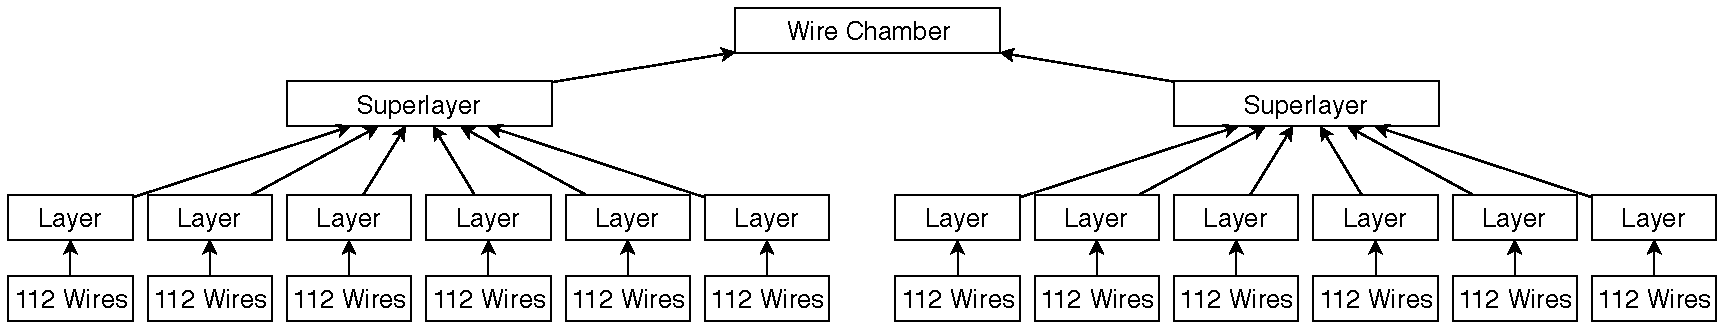
\includegraphics[width=\textwidth]{../figures/wire_chamber}
  \caption{The hierarchical structure of a single wire chamber.}
  \label{fig:wire-chamber}
\end{figure}

In order to gather as much information as possible on the particle
interactions, the 18 wire chambers are equally distributed across
three sectors within the drift chamber, the difference between the
sectors being their distance to the location of the electron beam hitting
the target. Sector one is located closest to the point of interest,
sector three is the furthest away.

\section{Drift Chamber Faults}

When conducting experiments, every part of the drift chamber
operates under extreme conditions, facing huge amounts of
radiation. Therefore, it is very common that
some components get damaged and stop working during the process. It
is crucial to spot these faults in time because the experimental
results strongly rely on the accuracy of the measurements.

Usually, faults occur within the scope of a single superlayer. To
visualize them, one can create a heatmap out of the wires' activations
that are accumulated during an experimental run, lighter areas
displaying higher activation than darker ones (see
Fig. \ref{fig:dead-wire} as an example). There are six different fault
types that can be distinguished:

\paragraph{Dead Wire:}
This fault occurs when a single wire
of a layer stops working, resulting in the wire displaying much lower
activations than its surroundings. An example of a dead wire is given
in Fig. \ref{fig:dead-wire}.

\paragraph{Dead Pin:}
A pin is composed of several successive
wires within a layer. See Fig. \ref{fig:dead-pin} for
an example of a dead pin.

\paragraph{Dead Connector:}
This component connects several wires
across a superlayer. If damaged, it results in a pattern of
activations that is illustrated in Fig. \ref{fig:dead-connector}.

\paragraph{Dead Fuse:}
A fuse is a collection of multiple
connectors, therefore the resulting fault pattern appears wider
than that of a dead connector.

\paragraph{Dead Channel:}
Multiple fuses can be connected within
a channel. This is the biggest fault that can appear within a
superlayer.

\paragraph{Hot Wire:}
This anomaly is quite different from the other faults. It occurs when
a single wire suddenly starts emitting huge amounts of activation,
silhouetting against the wires in its immediate surroundings. An
example of a hot wire can be seen in Fig. \ref{fig:hot-wire}.
\\
\\
The aim of this thesis is to develop a system that is capable of
recognizing faults occuring during an experimental run. In order to
achieve this, algorithms of artificial intelligence
and deep learning will be applied to the problem of fault detection. A
detailed description of the employed methods will
be delivered in the following chapters.

\begin{figure}[h]
  \centering
  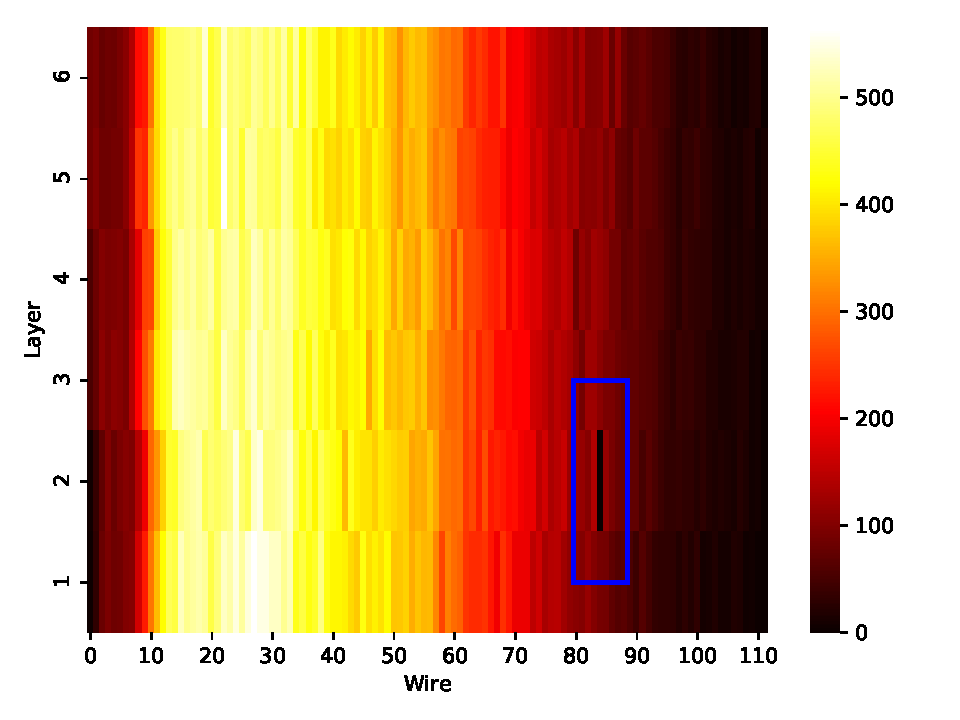
\includegraphics[width=\textwidth]{../figures/dead_wire}
  \caption{A single dead wire marked by the blue rectangle.}
  \label{fig:dead-wire}
\end{figure}

\begin{figure}
  \centering
  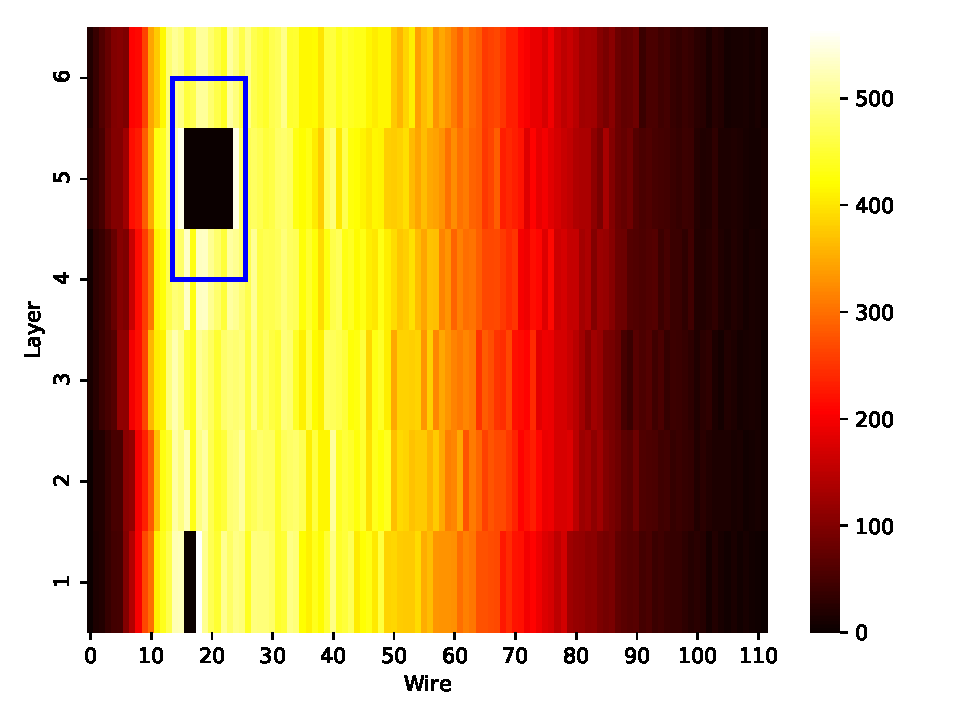
\includegraphics[width=\textwidth]{../figures/dead_pin}
  \caption{A dead pin spanning eight wires, marked by the blue
    rectangle. Also notice that
    there are two dead wires right next to each other in layer 1.}
  \label{fig:dead-pin}
\end{figure}

\begin{figure}
  \centering
  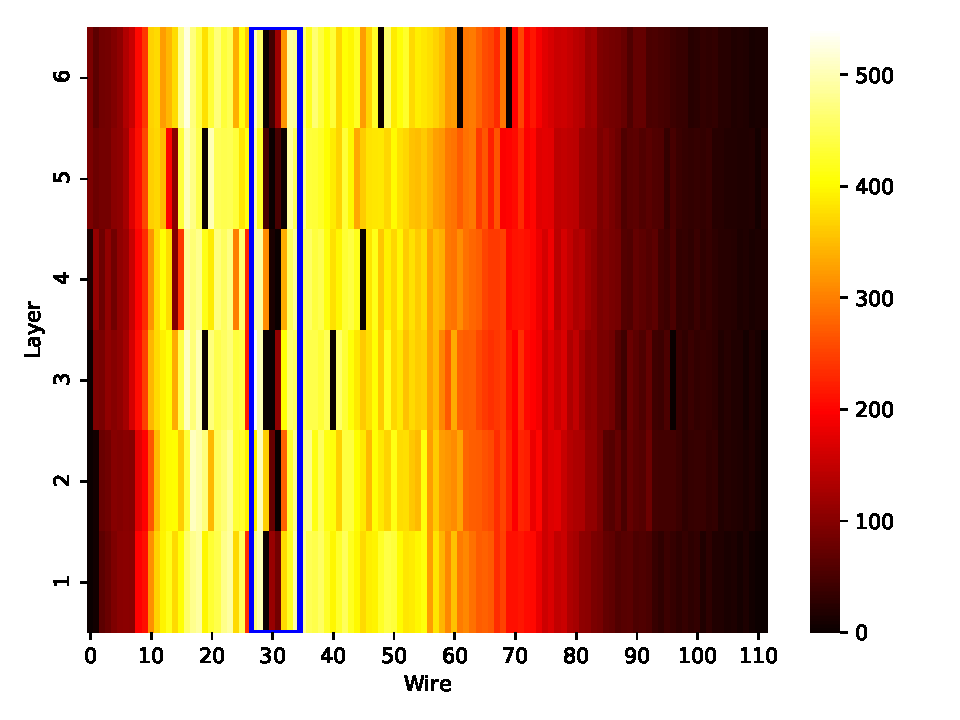
\includegraphics[width=\textwidth]{../figures/dead_connector}
  \caption{A dead connector surrounded by some dead wires.}
  \label{fig:dead-connector}
\end{figure}

\begin{figure}
  \centering
  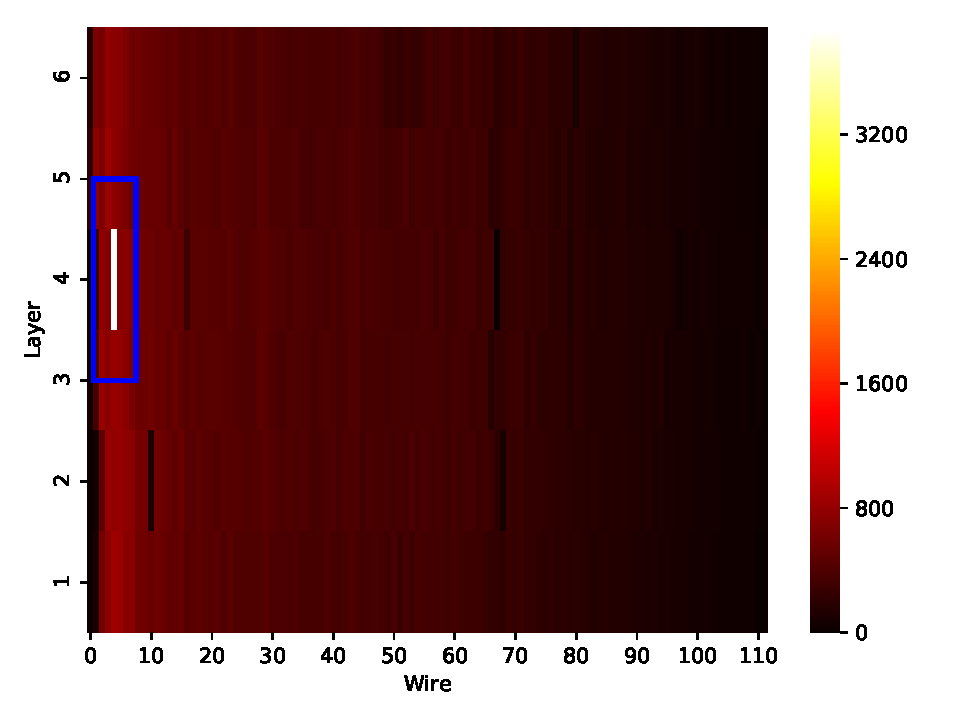
\includegraphics[width=\textwidth]{../figures/hot_wire}
  \caption{A hot wire displaying much more activation than its
    surrounding wires.}
  \label{fig:hot-wire}
\end{figure}

